\documentclass[aspectratio=169, 12pt]{beamer}
\usepackage{bbm}
\usepackage[utf8]{inputenc}
\usepackage[T2A]{fontenc}
\usepackage[english]{babel}
\usepackage{amscd,amssymb}
\usepackage{amsfonts,amsmath,array}
\usepackage{sidecap}
\usepackage{graphicx}
\DeclareGraphicsExtensions{.pdf,.png,.jpg}
\usepackage{pdfpages}
\usepackage{multicol}

\usepackage{amsthm}
\usepackage{mathtools}
\usepackage{algorithm}
\usepackage{algpseudocode}
\usepackage{color}
\usepackage{colortbl}
\usepackage{multirow}

\newtheorem{assumption}{Assumption}
\usetheme{boxes}



\title{Multiobjective Tree-Structured Parzen Estimator}
\author[V.\,M.~Meshkov]{Vladislav Meshkov, MSc.}
\institute{Moscow Institute of Physics and Technology}
\date{\today}

\begin{document}
\maketitle

\section{Motivation: Real-World Problems}
\begin{frame}
\frametitle{Motivation: Real-World Problems}
\begin{itemize}
\item Many real-world problems involve optimizing \textbf{multiple conflicting objectives} simultaneously
    
    Examples: 
    \begin{itemize}
        \item Mechanical design (diesel engine, air intake systems) requiring expensive CFD simulations
        \item Automated ML: high accuracy \textbf{vs.} low computational cost
    \end{itemize}

\item Objective functions are:
    \begin{itemize}
        \item \textbf{Expensive} to evaluate (time/money)
        \item \textbf{Black-box} (no analytical form)
        \item Defined on \textbf{complex/tree-structured} search spaces (mix of real, integer, categorical + conditional parameters)
    \end{itemize}

\item Need an algorithm that:
    \begin{itemize}
        \item Works with a \textbf{limited evaluation budget}
        \item Handles \textbf{complex search spaces} naturally
        \item Is \textbf{scalable} and \textbf{parallelizable}
    \end{itemize}
\end{itemize}
\end{frame}

\section{Limitations of Existing Methods}
\begin{frame}{Limitations of Existing Methods}

\textbf{Gaussian Process (GP)-based methods (PESMO, SMS-EGO, ParEGO):}
\begin{itemize}
    \item \textbf{De facto standard} in Bayesian optimization
    \item Provide uncertainty estimates for exploration/exploitation trade-off
    \item \alert{But:}
    \begin{itemize}
        \item Not suitable for non-continuous/conditional spaces
        \item High computational complexity \(O(n^3)\) — poor scalability
        \item Approximation techniques help but cause performance degradation
    \end{itemize}
\end{itemize}

\vspace{0.3cm}

\textbf{Tree-Structured Parzen Estimator (TPE):}
\begin{itemize}
    \item Non-GP surrogate (Parzen window density estimation)
    \item Naturally handles complex/conditional spaces
    \item Scales to \(\sim 1000\) observations, tens of variables
    \item Outperforms GP-based methods on single-objective HPO
    \item \alert{But:} Designed for \textbf{single-objective} only!
\end{itemize}

\vspace{0.2cm}

\end{frame}

\section{Formal Problem Statement}
\begin{frame}{Formal Problem Statement}

\textbf{Problem:}
\[
\underset{\mathbf{x} \in X}{\mathrm{minimize}} \quad \mathbf{f}(\mathbf{x}) := (f_1(\mathbf{x}), \ldots, f_m(\mathbf{x}))
\]

\vspace{0.2cm}

\textbf{Given:}
\begin{itemize}
    \item Tree-structured search space \(X = X_1 \times \ldots \times X_n\)
    \item Mixed variable types: real, integer, categorical
    \item Conditional variables (active only when parent takes specific values)
    \item Expensive black-box objectives \(f_j\)
\end{itemize}

\vspace{0.3cm}

\textbf{Goal:} Efficiently approximate the \textbf{Pareto front} with limited evaluation budget

\vspace{0.3cm}

\textbf{Dominance (minimization):}
\begin{itemize}
    \item \(y \prec y'\) iff \(\forall i: y_i \leq y_i'\) and \(\exists i: y_i < y_i'\)
    \item Pareto set: \(\{x \in X \mid \not\exists x' \in X: f(x') \prec f(x)\}\)
\end{itemize}

\end{frame}

\section{Background: TPE Algorithm}
\begin{frame}{Background: TPE for Single-Objective}

\textbf{Key Idea:} Model \(p(x_i \mid y)\) using two densities:
\[
p(x_i \mid y) = 
\begin{cases}
l(x_i) & \text{if } y < y^* \quad (\text{"good" observations})\\
g(x_i) & \text{if } y \geq y^* \quad (\text{"poor" observations})
\end{cases}
\]
where \(y^*\) is quantile threshold (\(p(y < y^*) = \gamma\))

\vspace{0.3cm}

\textbf{Acquisition Function (Expected Improvement):}
\[
\mathrm{EI}_{y^*}(x_i) \propto \left(\gamma + (1-\gamma)\frac{g(x_i)}{l(x_i)}\right)^{-1}
\]
\(\Rightarrow\) Maximize EI by maximizing ratio \(l(x_i)/g(x_i)\)

\vspace{0.3cm}

\textbf{Density Estimation (per parameter):}
\begin{itemize}
    \item Real/Integer: truncated Gaussian (adaptive bandwidth)
    \item Categorical: weighted histogram
    \item Conditional variables sampled from root to leaves
\end{itemize}

\end{frame}

\section{MOTPE: Key Contributions}
\begin{frame}{MOTPE: Key Contributions}

\textbf{Two Main Challenges in Extending TPE:}

\begin{enumerate}
    \item \textbf{Splitting observations} with multiple incomparable objectives
    \item \textbf{Multiobjective acquisition function} that drives Pareto front improvement
\end{enumerate}

\vspace{0.5cm}

\textbf{Solution Overview:}
\begin{itemize}
    \item \textbf{Split rule:} \(y \prec Y^*\) or \(y \parallel Y^*\) for \(l(x_i)\), \(Y^* \preceq y\) for \(g(x_i)\)
    \item \textbf{Greedy splitting:} Nondominated sorting + Hypervolume Subset Selection (HSSP)
    \item \textbf{Weighting:} Assign weights proportional to hypervolume contribution for \(l(x_i)\)
    \item \textbf{Acquisition:} Expected Hypervolume Improvement (EHVI) $\propto \left(\gamma + (1-\gamma)\frac{g}{l}\right)^{-1}$
\end{itemize}

\end{frame}

\section{MOTPE: Splitting Observations}
\begin{frame}{MOTPE: Splitting Observations (Algorithm 2)}

\textbf{Goal:} Select \(\lfloor \gamma |D| \rfloor\) observations for \(l(x_i)\) (good set)

\vspace{0.2cm}

\textbf{Greedy Algorithm:}
\begin{enumerate}
    \item Compute nondomination ranks (Pareto sorting)
    \item Greedily add full nondomination fronts while \(|D_l| + |D_{\text{rank}(j)}| \leq \lfloor \gamma |D| \rfloor\)
    \item For remaining slots, solve \textbf{Hypervolume Subset Selection Problem (HSSP)}
\end{enumerate}

\vspace{0.3cm}

\textbf{HSSP via Greedy (Algorithm 3):}
\begin{itemize}
    \item Find subset of size \(n_s\) maximizing hypervolume indicator
    \item Greedy algorithm gives \((1 - 1/e)\)-optimality guarantee (submodular maximization)
    \item Reference point: \((\max(y_1, y_1'), \ldots, \max (y_m, y_m'))\)
\end{itemize}

\vspace{0.3cm}

\textbf{Weighting:} \(w_j \propto\) hypervolume contribution for \(l(x_i)\), uniform weight 1 for \(g(x_i)\)
\end{frame}

\begin{frame}{MOTPE: Algorithm Overview (Algorithm 4)}

\textbf{Input:} Observations \(D\), quantile \(\gamma\), candidates \(n_c\)

\vspace{0.2cm}

\textbf{For each iteration:}
\begin{enumerate}
    \item Split \(D\) into \(D_l\) and \(D_g\) (Algorithm 2)
    \item \textbf{For each active parameter \(x_i\) (root to leaves):}
    \begin{itemize}
        \item Construct densities \(l(x_i)\) from \(D_l\), \(g(x_i)\) from \(D_g\)
        \item Sample \(n_c\) candidates from \(l(x_i)\)
        \item Select \(x_i^* = \mathrm{argmax} \, l(x_i)/g(x_i)\)
    \end{itemize}
    \item Evaluate \(f(x^*)\), add to \(D\)
\end{enumerate}

\vspace{0.3cm}

\textbf{Complexity:}
\begin{itemize}
    \item Memory: \(O(kn)\) where \(k\) = observations, \(n\) = parameters
    \item Time per iteration: \(O(k \log k + n_c \cdot n \cdot \text{cost}(l))\) 
    \item Much faster than GP-based methods (hours vs. days in experiments!)
\end{itemize}

\end{frame}



\section{Experimental Results}
\begin{frame}{Experiment 1: WFG Benchmark (Low Dim, Limited Budget)}

\textbf{Setup:} Comparison with GP-based methods (PESMO, ParEGO, SMS-EGO) on WFG problems.
\begin{center}
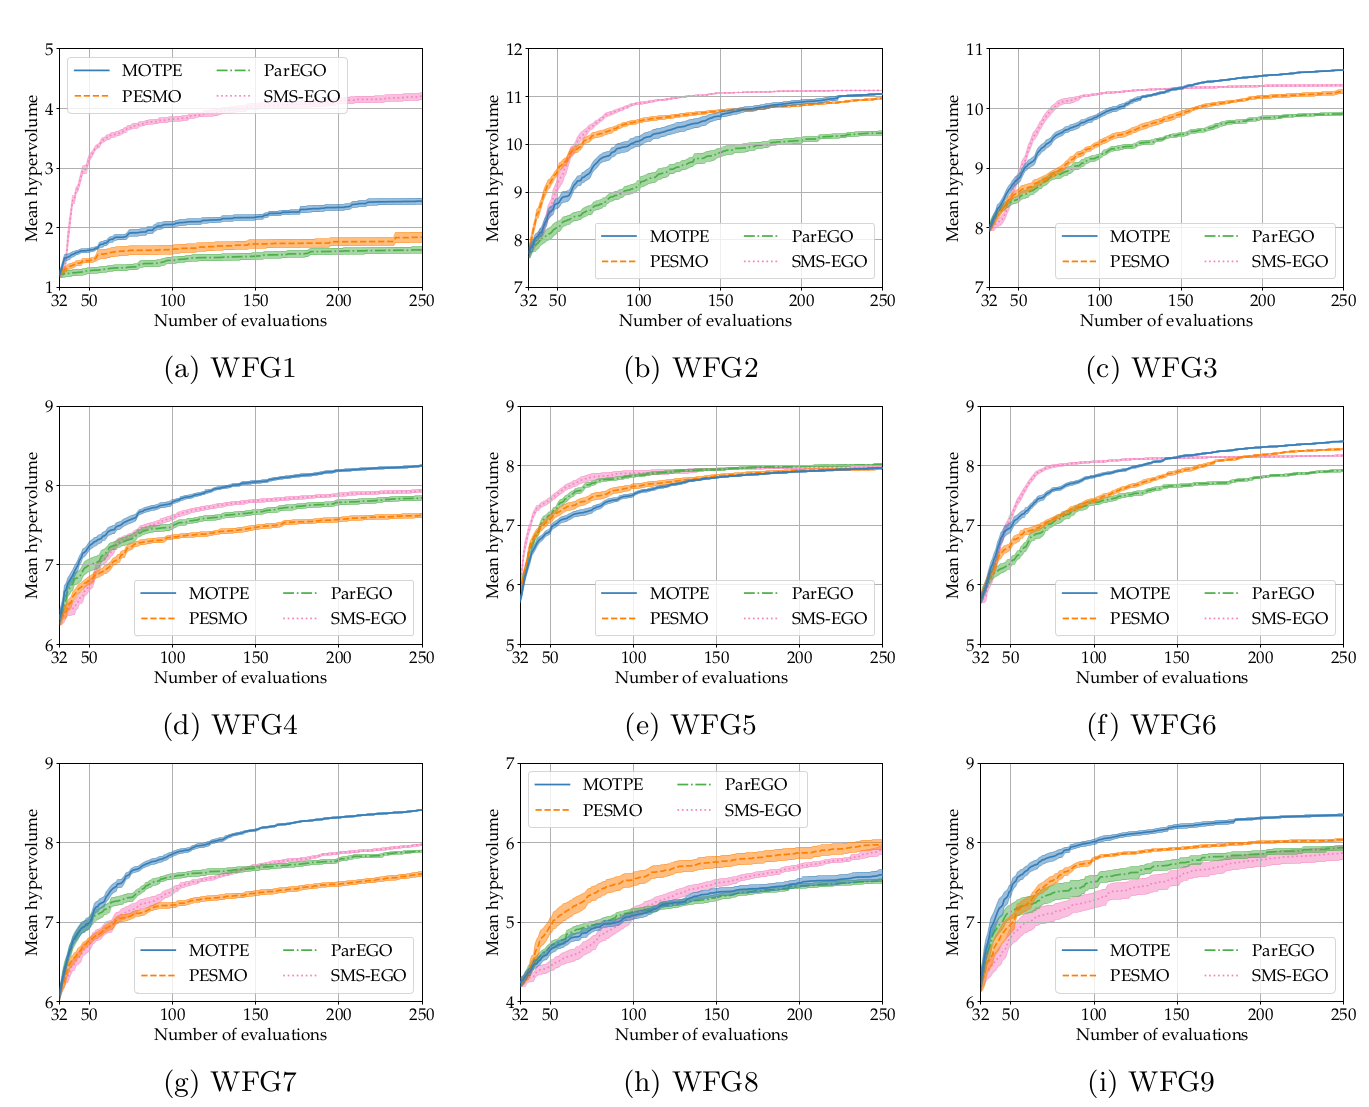
\includegraphics[width=0.6\textwidth]{figure_4.png}
\end{center}

\textbf{Key findings:}
\begin{itemize}
    \item MOTPE \textbf{outperforms} GP-based methods on most problems (WFG2-9)
    \item WFG1 (extremely biased) — difficult for all methods
    \item MOTPE robust to non-separability and multimodality
\end{itemize}
\end{frame}

\begin{frame}{Experiment 2: Real-World Problem — CNN Design}

\textbf{Task:} Design CNN for CIFAR-10 with two objectives:
\begin{enumerate}
    \item Minimize classification \textbf{error rate}
    \item Minimize \textbf{prediction time} (inference speed)
\end{enumerate}

\vspace{0.2cm}
\textbf{Search space:} 13 parameters (many conditional), including number of blocks, filters, batch norm, etc.

\begin{center}
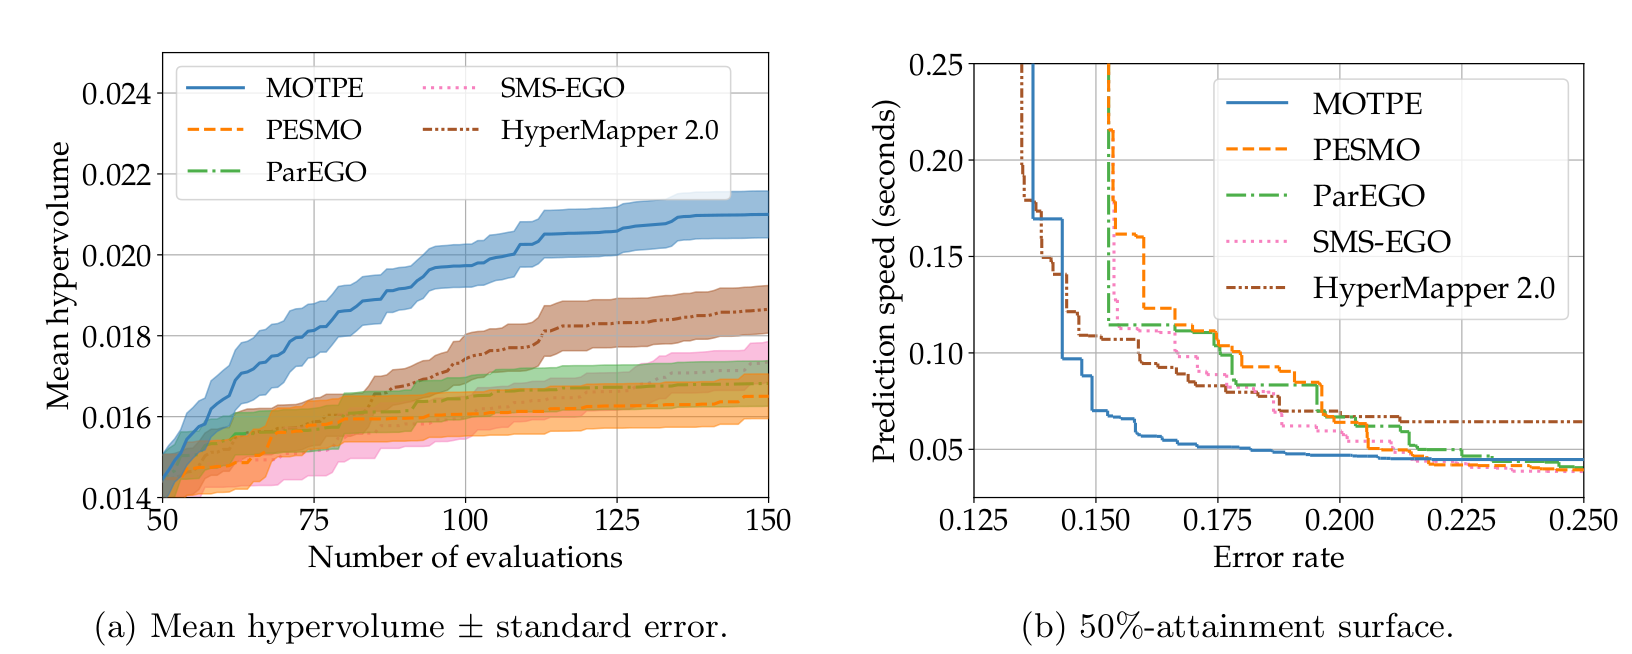
\includegraphics[width=0.7\textwidth]{figure_11.png}
\end{center}
\end{frame}

\end{document}